\subsection{Program master GBTx with external \itwoc adapter}
Before proceed, follow the instruction on \autoref{sec:hardware-ext-i2c} to
configure the hardware first.
As said in the previous section, the master GBTx board must be programmed via an
external \itwoc adapter first.
A Windows 7 computer on the rack is used. The \textbf{GBTX programmer} is
located at:

\begin{lstlisting}
DT_Rack\GBTx_programmer\GBTxProgrammer.jar
\end{lstlisting}

\begin{figure}[ht]
    \centering
    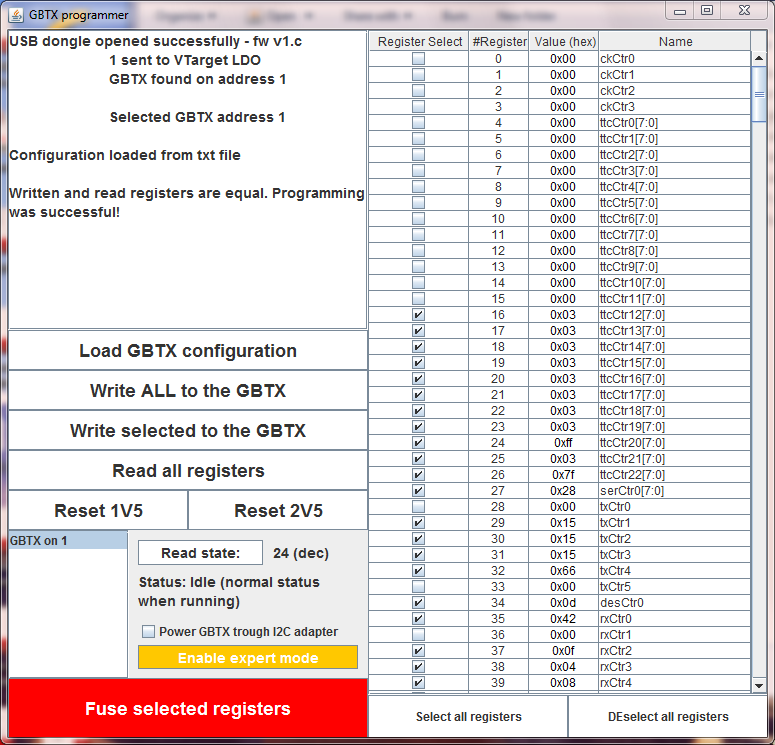
\includegraphics[width=0.9\textwidth]{res/gbtx_programmer_v1_ui.png}
    \caption{A typical UI for GBTX programmer.}
    \label{fig:gbtx-programmer-ui}
\end{figure}

Launch the programmer, a typical UI is shown in
\autoref{fig:gbtx-programmer-ui},
Click \textbf{Load GBTX configuration} and load a configuration file, which is
located at:

\begin{lstlisting}
Documents\master.txt
\end{lstlisting}

Then click \textbf{Write ALL to the GBTX}. Check the returned message to make
sure everything works (supposedly).
Now click \textbf{Read state}.
If the master GBTx is configured correctly and is connected to a working
MiniDAQ, the return value should be:

\begin{lstlisting}
24 (dec): Idle (normal status when running)
\end{lstlisting}
